%% bare_conf.tex
%% V1.4a
%% 2014/09/17
%% by Michael Shell
%% See:
%% http://www.michaelshell.org/
%% for current contact information.
%%
%% This is a skeleton file demonstrating the use of IEEEtran.cls
%% (requires IEEEtran.cls version 1.8a or later) with an IEEE
%% conference paper.
%%
%% Support sites:
%% http://www.michaelshell.org/tex/ieeetran/
%% http://www.ctan.org/tex-archive/macros/latex/contrib/IEEEtran/
%% and
%% http://www.ieee.org/

%%*************************************************************************
%% Legal Notice:
%% This code is offered as-is without any warranty either expressed or
%% implied; without even the implied warranty of MERCHANTABILITY or
%% FITNESS FOR A PARTICULAR PURPOSE! 
%% User assumes all risk.
%% In no event shall IEEE or any contributor to this code be liable for
%% any damages or losses, including, but not limited to, incidental,
%% consequential, or any other damages, resulting from the use or misuse
%% of any information contained here.
%%
%% All comments are the opinions of their respective authors and are not
%% necessarily endorsed by the IEEE.
%%
%% This work is distributed under the LaTeX Project Public License (LPPL)
%% ( http://www.latex-project.org/ ) version 1.3, and may be freely used,
%% distributed and modified. A copy of the LPPL, version 1.3, is included
%% in the base LaTeX documentation of all distributions of LaTeX released
%% 2003/12/01 or later.
%% Retain all contribution notices and credits.
%% ** Modified files should be clearly indicated as such, including  **
%% ** renaming them and changing author support contact information. **
%%
%% File list of work: IEEEtran.cls, IEEEtran_HOWTO.pdf, bare_adv.tex,
%%                    bare_conf.tex, bare_jrnl.tex, bare_conf_compsoc.tex,
%%                    bare_jrnl_compsoc.tex, bare_jrnl_transmag.tex
%%*************************************************************************


% *** Authors should verify (and, if needed, correct) their LaTeX system  ***
% *** with the testflow diagnostic prior to trusting their LaTeX platform ***
% *** with production work. IEEE's font choices and paper sizes can       ***
% *** trigger bugs that do not appear when using other class files.       ***                          ***
% The testflow support page is at:
% http://www.michaelshell.org/tex/testflow/



\documentclass[conference]{IEEEtran}
% Some Computer Society conferences also require the compsoc mode option,
% but others use the standard conference format.
%
% If IEEEtran.cls has not been installed into the LaTeX system files,
% manually specify the path to it like:
% \documentclass[conference]{../sty/IEEEtran}

\usepackage{amsmath}
\usepackage{blindtext, graphicx}
\usepackage{algorithm}

\usepackage{bbm}

\usepackage{algpseudocode}
\usepackage{pifont}
\usepackage{tikz}
\usepackage{amssymb}
%\usepackage{natbib}
\usepackage{upgreek}

\usepackage{mathtools}


% Some very useful LaTeX packages include:
% (uncomment the ones you want to load)


% *** MISC UTILITY PACKAGES ***
%
%\usepackage{ifpdf}
% Heiko Oberdiek's ifpdf.sty is very useful if you need conditional
% compilation based on whether the output is pdf or dvi.
% usage:
% \ifpdf
%   % pdf code
% \else
%   % dvi code
% \fi
% The latest version of ifpdf.sty can be obtained from:
% http://www.ctan.org/tex-archive/macros/latex/contrib/oberdiek/
% Also, note that IEEEtran.cls V1.7 and later provides a builtin
% \ifCLASSINFOpdf conditional that works the same way.
% When switching from latex to pdflatex and vice-versa, the compiler may
% have to be run twice to clear warning/error messages.






% *** CITATION PACKAGES ***
%
%\usepackage{cite}
% cite.sty was written by Donald Arseneau
% V1.6 and later of IEEEtran pre-defines the format of the cite.sty package
% \cite{} output to follow that of IEEE. Loading the cite package will
% result in citation numbers being automatically sorted and properly
% "compressed/ranged". e.g., [1], [9], [2], [7], [5], [6] without using
% cite.sty will become [1], [2], [5]--[7], [9] using cite.sty. cite.sty's
% \cite will automatically add leading space, if needed. Use cite.sty's
% noadjust option (cite.sty V3.8 and later) if you want to turn this off
% such as if a citation ever needs to be enclosed in parenthesis.
% cite.sty is already installed on most LaTeX systems. Be sure and use
% version 5.0 (2009-03-20) and later if using hyperref.sty.
% The latest version can be obtained at:
% http://www.ctan.org/tex-archive/macros/latex/contrib/cite/
% The documentation is contained in the cite.sty file itself.






% *** GRAPHICS RELATED PACKAGES ***
%
\ifCLASSINFOpdf
  % \usepackage[pdftex]{graphicx}
  % declare the path(s) where your graphic files are
  % \graphicspath{{../pdf/}{../jpeg/}}
  % and their extensions so you won't have to specify these with
  % every instance of \includegraphics
  % \DeclareGraphicsExtensions{.pdf,.jpeg,.png}
\else
  % or other class option (dvipsone, dvipdf, if not using dvips). graphicx
  % will default to the driver specified in the system graphics.cfg if no
  % driver is specified.
  % \usepackage[dvips]{graphicx}
  % declare the path(s) where your graphic files are
  % \graphicspath{{../eps/}}
  % and their extensions so you won't have to specify these with
  % every instance of \includegraphics
  % \DeclareGraphicsExtensions{.eps}
\fi
% graphicx was written by David Carlisle and Sebastian Rahtz. It is
% required if you want graphics, photos, etc. graphicx.sty is already
% installed on most LaTeX systems. The latest version and documentation
% can be obtained at: 
% http://www.ctan.org/tex-archive/macros/latex/required/graphics/
% Another good source of documentation is "Using Imported Graphics in
% LaTeX2e" by Keith Reckdahl which can be found at:
% http://www.ctan.org/tex-archive/info/epslatex/
%
% latex, and pdflatex in dvi mode, support graphics in encapsulated
% postscript (.eps) format. pdflatex in pdf mode supports graphics
% in .pdf, .jpeg, .png and .mps (metapost) formats. Users should ensure
% that all non-photo figures use a vector format (.eps, .pdf, .mps) and
% not a bitmapped formats (.jpeg, .png). IEEE frowns on bitmapped formats
% which can result in "jaggedy"/blurry rendering of lines and letters as
% well as large increases in file sizes.
%
% You can find documentation about the pdfTeX application at:
% http://www.tug.org/applications/pdftex





% *** MATH PACKAGES ***
%
%\usepackage[cmex10]{amsmath}
% A popular package from the American Mathematical Society that provides
% many useful and powerful commands for dealing with mathematics. If using
% it, be sure to load this package with the cmex10 option to ensure that
% only type 1 fonts will utilized at all point sizes. Without this option,
% it is possible that some math symbols, particularly those within
% footnotes, will be rendered in bitmap form which will result in a
% document that can not be IEEE Xplore compliant!
%
% Also, note that the amsmath package sets \interdisplaylinepenalty to 10000
% thus preventing page breaks from occurring within multiline equations. Use:
%\interdisplaylinepenalty=2500
% after loading amsmath to restore such page breaks as IEEEtran.cls normally
% does. amsmath.sty is already installed on most LaTeX systems. The latest
% version and documentation can be obtained at:
% http://www.ctan.org/tex-archive/macros/latex/required/amslatex/math/





% *** SPECIALIZED LIST PACKAGES ***
%
%\usepackage{algorithmic}
% algorithmic.sty was written by Peter Williams and Rogerio Brito.
% This package provides an algorithmic environment fo describing algorithms.
% You can use the algorithmic environment in-text or within a figure
% environment to provide for a floating algorithm. Do NOT use the algorithm
% floating environment provided by algorithm.sty (by the same authors) or
% algorithm2e.sty (by Christophe Fiorio) as IEEE does not use dedicated
% algorithm float types and packages that provide these will not provide
% correct IEEE style captions. The latest version and documentation of
% algorithmic.sty can be obtained at:
% http://www.ctan.org/tex-archive/macros/latex/contrib/algorithms/
% There is also a support site at:
% http://algorithms.berlios.de/index.html
% Also of interest may be the (relatively newer and more customizable)
% algorithmicx.sty package by Szasz Janos:
% http://www.ctan.org/tex-archive/macros/latex/contrib/algorithmicx/




% *** ALIGNMENT PACKAGES ***
%
%\usepackage{array}
% Frank Mittelbach's and David Carlisle's array.sty patches and improves
% the standard LaTeX2e array and tabular environments to provide better
% appearance and additional user controls. As the default LaTeX2e table
% generation code is lacking to the point of almost being broken with
% respect to the quality of the end results, all users are strongly
% advised to use an enhanced (at the very least that provided by array.sty)
% set of table tools. array.sty is already installed on most systems. The
% latest version and documentation can be obtained at:
% http://www.ctan.org/tex-archive/macros/latex/required/tools/


% IEEEtran contains the IEEEeqnarray family of commands that can be used to
% generate multiline equations as well as matrices, tables, etc., of high
% quality.




% *** SUBFIGURE PACKAGES ***
%\ifCLASSOPTIONcompsoc
%  \usepackage[caption=false,font=normalsize,labelfont=sf,textfont=sf]{subfig}
%\else
%  \usepackage[caption=false,font=footnotesize]{subfig}
%\fi
% subfig.sty, written by Steven Douglas Cochran, is the modern replacement
% for subfigure.sty, the latter of which is no longer maintained and is
% incompatible with some LaTeX packages including fixltx2e. However,
% subfig.sty requires and automatically loads Axel Sommerfeldt's caption.sty
% which will override IEEEtran.cls' handling of captions and this will result
% in non-IEEE style figure/table captions. To prevent this problem, be sure
% and invoke subfig.sty's "caption=false" package option (available since
% subfig.sty version 1.3, 2005/06/28) as this is will preserve IEEEtran.cls
% handling of captions.
% Note that the Computer Society format requires a larger sans serif font
% than the serif footnote size font used in traditional IEEE formatting
% and thus the need to invoke different subfig.sty package options depending
% on whether compsoc mode has been enabled.
%
% The latest version and documentation of subfig.sty can be obtained at:
% http://www.ctan.org/tex-archive/macros/latex/contrib/subfig/




% *** FLOAT PACKAGES ***
%
%\usepackage{fixltx2e}
% fixltx2e, the successor to the earlier fix2col.sty, was written by
% Frank Mittelbach and David Carlisle. This package corrects a few problems
% in the LaTeX2e kernel, the most notable of which is that in current
% LaTeX2e releases, the ordering of single and double column floats is not
% guaranteed to be preserved. Thus, an unpatched LaTeX2e can allow a
% single column figure to be placed prior to an earlier double column
% figure. The latest version and documentation can be found at:
% http://www.ctan.org/tex-archive/macros/latex/base/


%\usepackage{stfloats}
% stfloats.sty was written by Sigitas Tolusis. This package gives LaTeX2e
% the ability to do double column floats at the bottom of the page as well
% as the top. (e.g., "\begin{figure*}[!b]" is not normally possible in
% LaTeX2e). It also provides a command:
%\fnbelowfloat
% to enable the placement of footnotes below bottom floats (the standard
% LaTeX2e kernel puts them above bottom floats). This is an invasive package
% which rewrites many portions of the LaTeX2e float routines. It may not work
% with other packages that modify the LaTeX2e float routines. The latest
% version and documentation can be obtained at:
% http://www.ctan.org/tex-archive/macros/latex/contrib/sttools/
% Do not use the stfloats baselinefloat ability as IEEE does not allow
% \baselineskip to stretch. Authors submitting work to the IEEE should note
% that IEEE rarely uses double column equations and that authors should try
% to avoid such use. Do not be tempted to use the cuted.sty or midfloat.sty
% packages (also by Sigitas Tolusis) as IEEE does not format its papers in
% such ways.
% Do not attempt to use stfloats with fixltx2e as they are incompatible.
% Instead, use Morten Hogholm'a dblfloatfix which combines the features
% of both fixltx2e and stfloats:
%
% \usepackage{dblfloatfix}
% The latest version can be found at:
% http://www.ctan.org/tex-archive/macros/latex/contrib/dblfloatfix/




% *** PDF, URL AND HYPERLINK PACKAGES ***
%
%\usepackage{url}
% url.sty was written by Donald Arseneau. It provides better support for
% handling and breaking URLs. url.sty is already installed on most LaTeX
% systems. The latest version and documentation can be obtained at:
% http://www.ctan.org/tex-archive/macros/latex/contrib/url/
% Basically, \url{my_url_here}.




% *** Do not adjust lengths that control margins, column widths, etc. ***
% *** Do not use packages that alter fonts (such as pslatex).         ***
% There should be no need to do such things with IEEEtran.cls V1.6 and later.
% (Unless specifically asked to do so by the journal or conference you plan
% to submit to, of course. )


% correct bad hyphenation here
\hyphenation{Smart grids}

\begin{document}

%
% paper title
% Titles are generally capitalized except for words such as a, an, and, as,
% at, but, by, for, in, nor, of, on, or, the, to and up, which are usually
% not capitalized unless they are the first or last word of the title.
% Linebreaks \\ can be used within to get better formatting as desired.
% Do not put math or special symbols in the title.

\title{Multi-agent Q-Learning for minimizing Demand-Supply deficit in microgrids}


% author names and affiliations
% use a multiple column layout for up to three different
% affiliations

\author{\IEEEauthorblockN{Raghuram Bharadwaj D.}
	\IEEEauthorblockA{IISc, Bangalore, India\\
	 raghu.bharadwaj@csa.iisc.ernet.in}
	\and
	\IEEEauthorblockN{D. Sai Koti Reddy }
	\IEEEauthorblockA{IISc, Bangalore, India \\
		 danda.reddy@csa.iisc.ernet.in}
	\and
  \centering	\IEEEauthorblockN{Shalabh Bhatnagar}
	\IEEEauthorblockA{IISc, Bangalore, India\\
		shalabh@csa.iisc.ernet.in}}

%\author{Raghuram$^\dagger$, D. Sai Koti Reddy$^\dagger$,  Shalabh Bhatnagar$^\dagger$
%\thanks{
%$^\dagger$ Department of Computer Science and Automation,
%Indian Institute of Science, Bangalore,
%E-Mail: danda.reddy@csa.iisc.ernet.in, shalabh@csa.iisc.ernet.in}
%}

%\author{\IEEEauthorblockN{Raghuram}
%\IEEEauthorblockA{Department of Computer Science and Automation\\
%Indian Institute of Science, Bangalore\\
%Bangalore, India \\
%Email: http://www.michaelshell.org/contact.html}
%\and
%\IEEEauthorblockN{D. Sai Koti Reddy}
%\IEEEauthorblockA{Department of Computer Science and Automation\\
%Indian Institute of Science, Bangalore\\
%Bangalore, India \\
%Email: danda.reddy@csa.iisc.ernet.in}
%\and
%\IEEEauthorblockN{Shalabh Bhatnagar}
%\IEEEauthorblockA{Department of Computer Science and Automation\\
%Indian Institute of Science, Bangalore\\
%Bangalore, India \\
%Email: shalabh@csa.iisc.ernet.in}
%}



% conference papers do not typically use \thanks and this command
% is locked out in conference mode. If really needed, such as for
% the acknowledgment of grants, issue a \IEEEoverridecommandlockouts
% after \documentclass

% for over three affiliations, or if they all won't fit within the width
% of the page, use this alternative format:
% 
%\author{\IEEEauthorblockN{Michael Shell\IEEEauthorrefmark{1},
%Homer Simpson\IEEEauthorrefmark{2},
%James Kirk\IEEEauthorrefmark{3}, 
%Montgomery Scott\IEEEauthorrefmark{3} and
%Eldon Tyrell\IEEEauthorrefmark{4}}
%\IEEEauthorblockA{\IEEEauthorrefmark{1}School of Electrical and Computer Engineering\\
%Georgia Institute of Technology,
%Atlanta, Georgia 30332--0250\\ Email: see http://www.michaelshell.org/contact.html}
%\IEEEauthorblockA{\IEEEauthorrefmark{2}Twentieth Century Fox, Springfield, USA\\
%Email: homer@thesimpsons.com}
%\IEEEauthorblockA{\IEEEauthorrefmark{3}Starfleet Academy, San Francisco, California 96678-2391\\
%Telephone: (800) 555--1212, Fax: (888) 555--1212}
%\IEEEauthorblockA{\IEEEauthorrefmark{4}Tyrell Inc., 123 Replicant Street, Los Angeles, California 90210--4321}}




% use for special paper notices
%\IEEEspecialpapernotice{(Invited Paper)}




% make the title area
\maketitle

% As a general rule, do not put math, special symbols or citations
% in the abstract
\begin{abstract}

We consider the problem of minimizing the difference in the demand and the supply of the power using microgrids. We setup multiple microgrids, that provides electricity to a village. It has access to the batteries that can store renewable power and also the electrical lines from the main grid. At each time period, these microgrids need to take decision on amount of renewable power to be used from the batteries and amount of power needed from main grid. We formuate this problem in the framework of Markov Decision Process (MDP). The power allotment to the village from the main grid is fixed and bounded, whereas the renewable energy generation is uncertain in nature. Therefore we apply popular Reinforcement learning technique, Multi-Agent Q-Learning to solve this problem. Finally we consider a variant of this problem, where the cost of power production at main site is also included. In this scenario, the microgrids need to minimize the demand-supply deficit, while maintaining the desired average cost of the power production. 



\end{abstract}

% no keywords




% For peer review papers, you can put extra information on the cover
% page as needed:
% \ifCLASSOPTIONpeerreview
% \begin{center} \bfseries EDICS Category: 3-BBND \end{center}
% \fi
%
% For peerreview papers, this IEEEtran command inserts a page break and
% creates the second title. It will be ignored for other modes.
\IEEEpeerreviewmaketitle



\section{Introduction}

Electricity is one of the most important components of the modern life. There are a total of 18,452 unelectrified villages in India. Providing electricity to these villages is difficult for a number of reasons. The village may be situated very far away from the main grid and it would be difficult to establish a direct electrical line between them. Also, due to increasing global warming, we want to make less use of fossil fuels. Our objective in this work is to provide a solution to electrifying these villages.

We setup microgrids closer to the villages, with an electricity connection from main grids. The microgrids will also be provided with batteries that can store renewable energy sources. Owing to the cost, these batteries will have limited storage capacities. Now each microgrid needs to take decision on amount of renewable energy that needs to be used at every time slot and the amount of power that needs to drawn from the main grid. Consider a scenario where, microgrids will use the renewable energy as it is. That is, they do not store the energy. Then, during the peak demand, if the amount of renewable energy generated is low and power obtained from the main grid is also low, it leads to huge blackout. Thus, it is important to intelligently store and use the renewable energy. In this work, we apply Multi-agent Q-learning algorithm to solve this problem. 

-------Literature Work to Follow------------------

% \subsection{Subsection Heading Here}
% Subsection text here.


% \subsubsection{Subsubsection Heading Here}
% Subsubsection text here.

\section{Our Work}
In this section, we discuss two important problems associated with the microgrids. We first formulate the problem in the framework of Markov Decision Process (MDP), similar to the one described in \cite{goodmdp}. We then apply cooperative Multi-Agent Q-Learning algorithm to solve the problems.

\subsection{Problem 1 - Minimizing Demand-Supply Deficit}

Consider a village that has not been electrified yet. We setup microgrids close to the village, which provides electrical connections to the village. It also has connections from the main grid. Power supply is generally done in time slots, for example every 2 hours. Microgrids do not have non-renewable power generation capabilities. They have access to renewable power and needs to obtain excess power from main grid. For ease of explanation, we consider two renewable sources - solar and wind. At the beginning of each time slot, microgrids obtain the power demand from customers with the help of smart meters. These microgrids need to take decisions on amount of renewable power to be used so that the expected long term demand-supply deficit is minimized.

One natural solution without the use of storage batteries is to fully use the solar and wind power generated at every time slot. The excess demand will be then requested from the main grid. If the requested power is less than or equal to the maximum alloted power, the main grid transfers this to the microgrids. Other wise, it transfers the maximum alloted power. This idea is described in Algorithm 1.


\begin{algorithm}
\caption{}
\label{greedy}
\begin{algorithmic}[1]
	\State Demand $\leftarrow$ Initial Demand
    \State get\_Demand(Demand) : Procedure that gives next Demand level based on the current Demand level.
    \State solar() : Function that computes solar power generated in a time slot
    \State wind() : Function that computes wind power generated in a time slot
    \State max\_prod : Maximum power alloted by the main grid.
    \State Deficit = 0 ; iterations = 0
    \Procedure{At every Time Slot}{}   
     \State solar\_action = solar()
     \State wind\_action = wind()
     \State main\_action = max(0,min(max\_prod, Demand - (solar\_action+wind\_action)))
     \State Demand $\leftarrow$ get\_Demand(Demand).
     \State Deficit += Demand - (solar\_action + wind\_action + main\_action)
     \State iterations += 1;
    \EndProcedure
    \State Average Deficit = Deficit/iterations;
    
\end{algorithmic}
\end{algorithm}


Our objective in current work is to do better than the above described solution. We consider microgrids, equipped with the batteries that can store renewable power. That is, we deploy microgrids at the sites where there is availability of renewable resources. The goal is to intelligently use the stored power in batteries and take optimal action at every time slot to minimize the demand-supply deficit.

We formulate the problem in the framework of Markov Decision Process (MDP). MDP \cite{sutton} is the most popular mathematical framework for modeling optimal sequential decision making problems under uncertainty. A Markov decision process is defined via tuple $< S; A; P;R >$, where S is the set of states. A is the set of actions. P respectively the probability transition matrix. $P_{a}(s,s^{'})$ is the probability that action $a$ in state $s$, result into state $s^{'}$. R is the reward function where $R_{a}(s,s^{'})$ is the reward obtained by taking action $a$ in state $s$ and $s^{'}$ being the next state. In infinite cost discounted setting \cite{vol1}, the goal is to obtain a policy $\pi$, which is a mapping from state space to action space that maximizes the following objective:

\begin{equation}
\sum_{t = 0}^{\infty} \gamma^{t}R_{a_{t}}(s_{t},s_{t+1}),
\end{equation}
where $a_{t} = \pi(s_{t}),$ and $\gamma$ is the discount factor.

We model Power Demand as a Markov process. That is, current Demand depends only on the previous value. The Demand value, and the amount of power left in the batteries form the state of the MDP. That is, 
\begin{equation}
 state = [Demand, solar\_batterylevel, wind\_batterylevel].
\end{equation}

Based on the current state, the microgrids need to take action on number of units of power needs to be used from their batteries, and amount of power that is needed from the main grid. Note that the power from the main grid is fixed and bounded at all time periods, while power from renewable sources is uncertain in nature. 

\begin{equation}
Action = [solar\_power,wind\_power,main\_power],
\end{equation}

The state evolves as follows:
\begin{equation}
\begin{split}
solar\_batterylevel &= solar\_batterylevel - solar\_power \\&\hspace{1cm}+ solar(), 
\end{split}
\end{equation}
and
\begin{equation}
\begin{split}
wind\_batterylevel &= wind\_batterylevel - wind\_power 
\\&\hspace{1cm}  + wind(),
\end{split}
\end{equation}
where
$solar()$ and $wind()$ are the solar and wind power generation policies. 
Our objective is to minimize the long term average difference in demand and supply of the power. So, single stage Reward function is as follows:
%$$ Single\_stage\_cost\_function  =$$
\begin{equation}
\begin{split}
R = -&(Demand - \\
&(solar\_power+wind\_power+main\_power))^2
\end{split}
\end{equation}
When there is uncertainty in the system, like the renewal energy generation in this case, tradition solution techniques like Value iteration and policy iterations cannot be applied. Reinforcement Learning provides us with algorithms which can be applied when the model information is not completely known. One such popular model-free algorithm is Q-learning \cite{vol2}. However, we cannot have microgrids applying Q-Learning independently, as they are working towards a common goal. Hence we apply co-operative Multi-Agent Q-Learning algorithm \cite{marl} to solve the problem. At every slot, the microgrids exchange the battery level information among themselves. Then they apply Q-Learning on the joint state and obtain joint action. Each microgrid then selects its respective action. Let the joint state at time $k$ be $s_{k}$. We select a joint action, based on a $\epsilon-$greedy policy. Let it be $a_{k}$ and so we move to a new state $s_{k+1}$. Let the single stage reward obtained be $r_{k}$ Then the Q-values are updated as follows:
\begin{equation}\label{Q-val}
\begin{split}
Q(s_{k},a_{k}) = Q(s_{k},a_{k}) + \\
 \alpha[r_{k}+\gamma max_{a}Q(s_{k+1},a) - Q(s_{k},a_{k})] 
\end{split}
\end{equation}
We update this Q-values until convergence. At the end of this process, we will have an optimal policy that gives for each state, the optimal action to be taken. The idea is described in  Algorithm 2. 

\begin{algorithm}
\caption{}
\label{q-learning}
\begin{algorithmic}[1]
	\State  State $\leftarrow$ Initial State 
    \State get\_Demand(Demand) : Procedure that gives next Demand level based on the current Demand level.
   \State solar() : Function that computes solar power generated in a time slot
    \State wind() : Function that computes wind power generated in a time slot.
    \State max\_prod : Maximum power alloted by the main grid.
    \State Deficit = 0 ; iterations = 0
    \Procedure{At every Time Slot and for all the microgrids}{}   
     
     \State Select an joint action $a$ vector according to $\epsilon$-greedy policy.
     \State new\_solar = solar - a(solar\_action) + solar()
     \State new\_wind = wind - a(wind\_action) + wind()
     \State new\_Demand = get\_Demand(Demand)
     \State Update the Q-values according to \eqref{Q-val}
     \State state = [new\_Demand, new\_solar, new\_wind]
     \State Deficit += Demand - (a(solar\_action) + a(wind\_action) + a(main\_action))
     \State iterations += 1;
    \EndProcedure
    \State Average Deficit = Deficit/iterations;
\end{algorithmic}
\end{algorithm}


\subsection{Problem 2 - Balancing Demand-Supply Deficit and cost of Power Production}
In the above formulation, the cost of non-renewable power production at the main grid site is not taken into consideration. Therefore, it is natural to use the entire power obtained from the main grid and the optimization is done on the amount of power drawn from the solar and wind batteries. In this formulation, we put a cost on amount of power that can be obtained from the main grid. That is, we modify our single stage Reward as follows:
\begin{equation}\label{prob2}
\begin{split}
 -c*(Demand - (solar\_power + wind\_power+ \\
 main\_power))^2+(1-c)*(main\_power)^2.\\
 c \in[0,1],
 \end{split}
\end{equation}


where $c$ is the parameter that controls the demand-supply objective and the main grid production cost. 
Similar to the above problem, we apply multi-agent Q-Learning to obtain the optimal solution. 

\section{Experiments}
We consider 2 microgrids operating on solar and wind power batteries respectively. Demand values are taken to be 8,10 and 12. The probability transition matrix for the Demand levels is given below. 

$$ P = [0.1\hspace{0.1cm}0.6\hspace{0.1cm} 0.3; 0.3\hspace{0.1cm} 0.1\hspace{0.1cm} 0.6; 0.6 \hspace{0.1cm}0.3 \hspace{0.1cm}0.1];$$

The maximum storage capacity of the batteries is set to 5. The renewable energy generation process, for simulation purposes is considered to be Poisson with mean 2. Discount factor of the Q-learning is taken to be 0.9.

We begin our simulations with the state $[8,5,5]$. First we run Algorithm 1 for $10^6$ iterations and compute the average deficit in demand and the supply. Then we run Algorithm 2 for $10^8$ iterations and compute the average deficit using optimal Q-values for $10^4$ iterations. We compare both the algorithms in Figure 1.

\begin{figure}[h!]
\begin{center}
 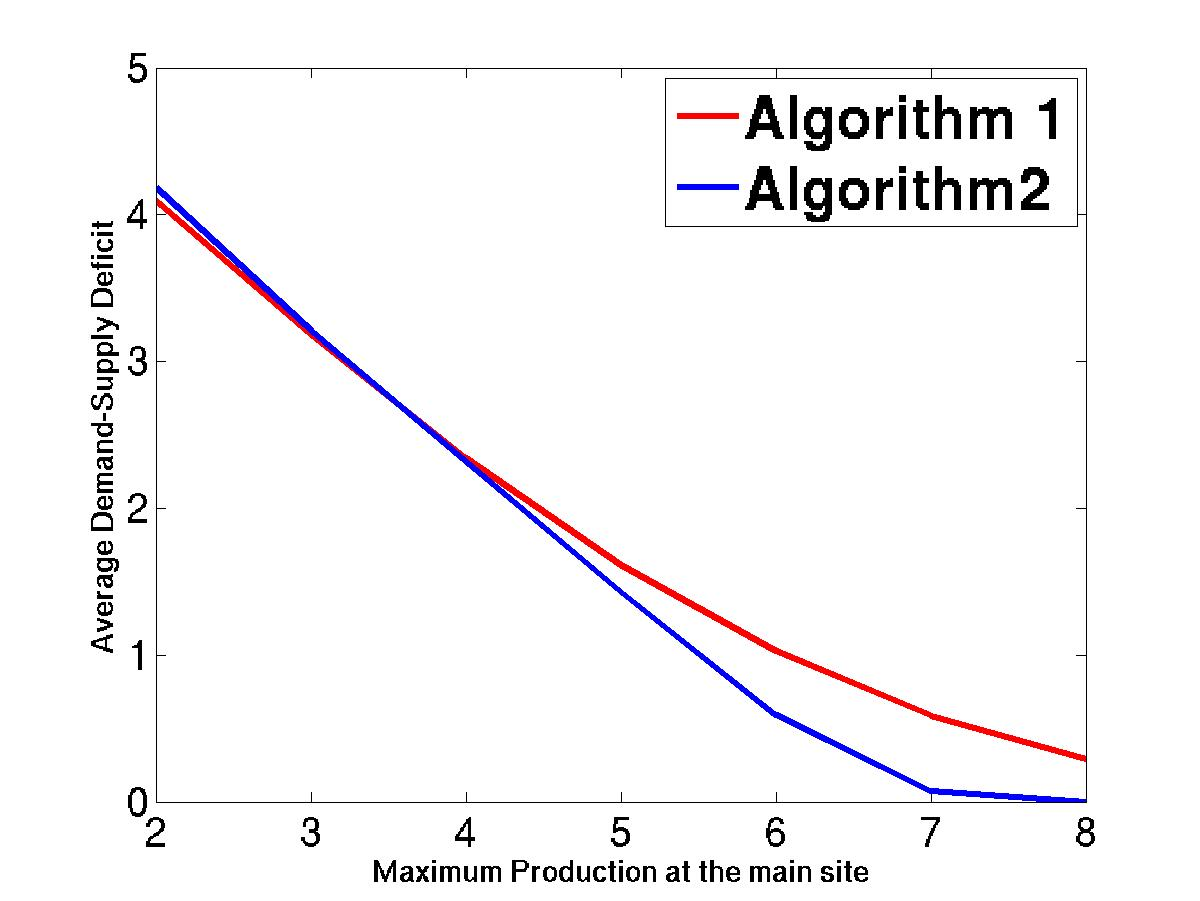
\includegraphics[width = 10cm,height=10cm]{plot1.jpg}
 \caption{Comparison of Algorithms on Problem 1}
 \end{center}
 \end{figure}


With regard to the problem 2, we plot the values of average deficit in the power and the average production at the main grid obtained by different values of $c$ in \eqref{prob2}. The maximum power allocation at the main site is set to 8. This is shown in Figure 2. 

\begin{figure}[h!]
\begin{center}
 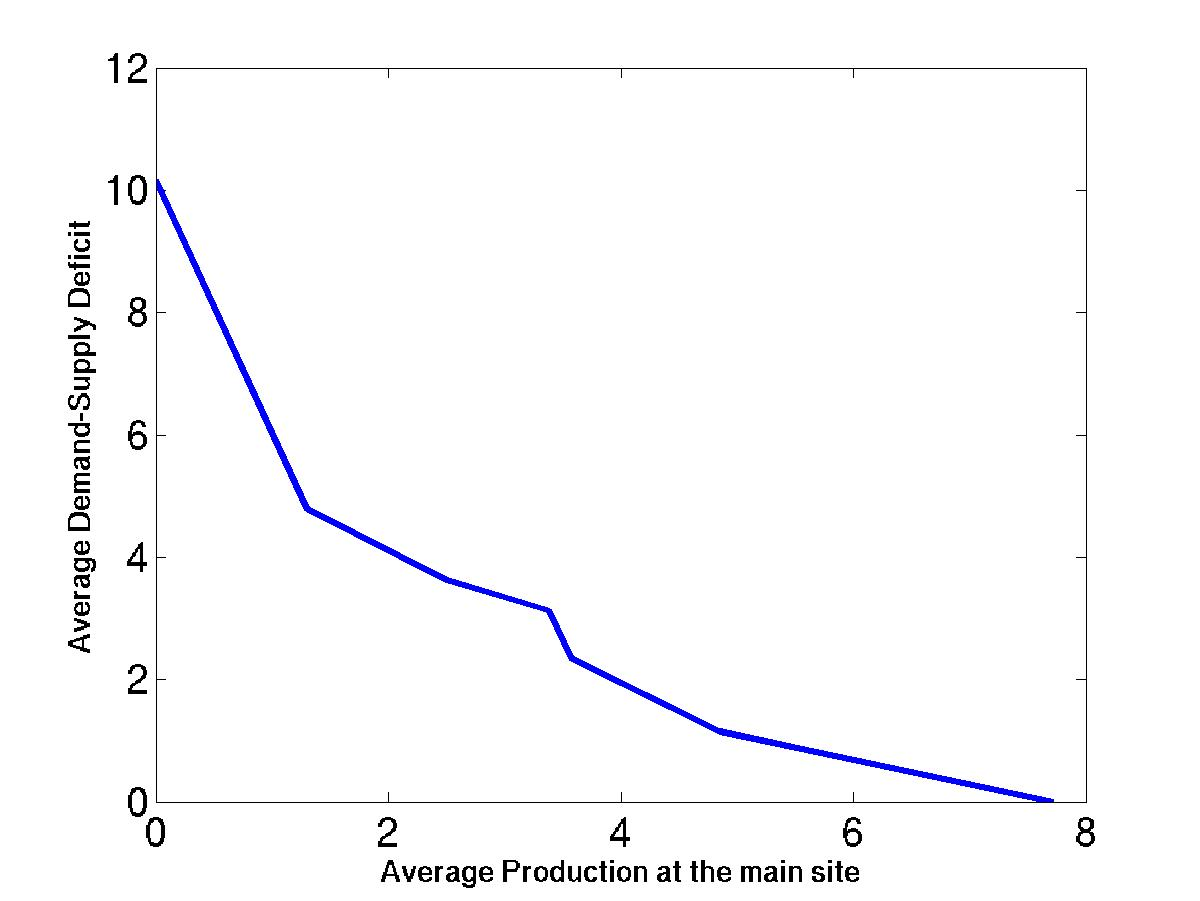
\includegraphics[width = 10cm,height=10cm]{plot2.jpg}
 \caption{Algorithm 2 applied to Problem 2}
 \end{center}
 \end{figure}

\subsection{Observations}

\begin{itemize}
\item In Figure 1, we see that Algorithm 1 performs better than Algorithm 2, when the Maximum Power Allocation (MPA) at the main site is less than 3. This is because, when the MPA is very less compared to the minimum demand, storing the power in the batteries doesn't provide any advantage. 
\item On the other hand, if the MPA is closer to the minimum demand, Algorithm 2 outperforms Algorithm 1. 
\item In Figure 2, we observe that as the value of $c$ increases, average demand-supply deficit decreases and the average power obtained from the main grid increases. 
\end{itemize}



\section{Conclusion}
We considered the problem of electrifying a village by setting up microgrids close to the village. These have access to renewable energy storage batteries and also connections from the main grid. We identified two problems associated with the microgrid. One problem is to minimize the long-run discounted demand-supply deficit. We model this problem in the framework of MDP. This formulation doesn't take into consideration the cost of power production at the main grid site. Finally, we formulated MDP taking this in to consideration. We applied Multi-Agent Q-Learning algorithm to solve these problems. Simulations show that ....

\section{Future Work}
In Future, we would like to consider the possibility of power sharing between the microgrids. In this case, along with decision on amount to be used from stored batteries, microgrids also have to take decision on amount of power that can be shared with others. We would also like to include heterogeneous price system. In this scenario, price of power production at main grid varies from time to time.





% conference papers do not normally have an appendix


% use section* for acknowledgment
\section*{Acknowledgment}


The authors would like to thank...


 \bibliographystyle{IEEEtran}
 \bibliography{IEEEabrv,reference}




% that's all folks
\end{document}